\documentclass[../../main]{subfiles}
\begin{document}

\subsection{Live events}
\label{ss:final-live}

A live event is almost similar to a \textit{poi} but it has an expiration date that needs to be specified during its creation.
Live events are always public and available to the actual owner and their friends automatically.
On a live event dialog showing its details, no website URL or address are shown.
Instead, the expiration date and the actual owner are.
The images below show the dialog for the creation of a live event and the dialog for retrieving details about a live event.
\begin{figure}[H]
    \centering
    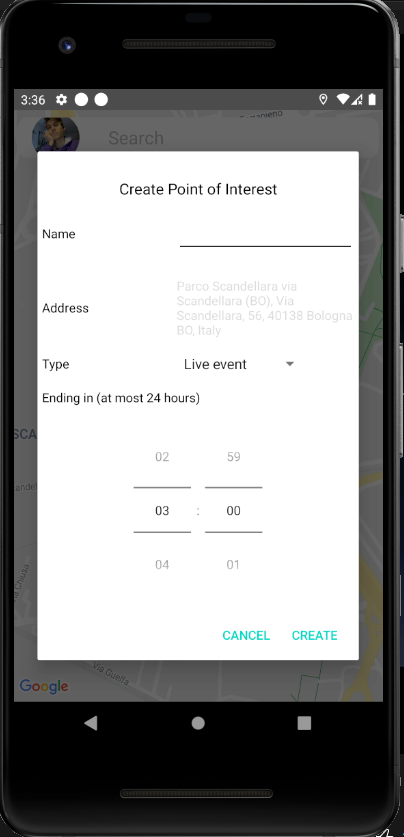
\includegraphics[width=0.41\textwidth]{images/app/live/creazione_live}
    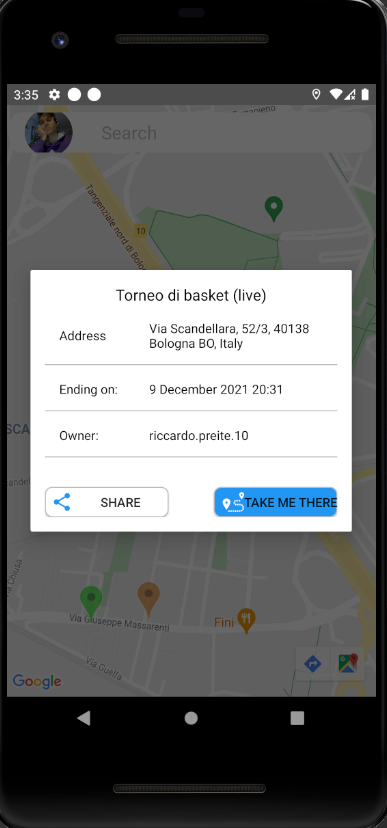
\includegraphics[width=0.4\textwidth]{images/app/live/live_map_detail}
    \caption{On the left, the dialog for creating a live event. On the right, the dialog with details about a live event.}
\end{figure}
\noindent
Users are notified when one of their friends add a live event.
Moreover, they can see all the live events not yet expired by navigating to the \textbf{Live events} screen from the main menu.
\begin{figure}[H]
    \centering
    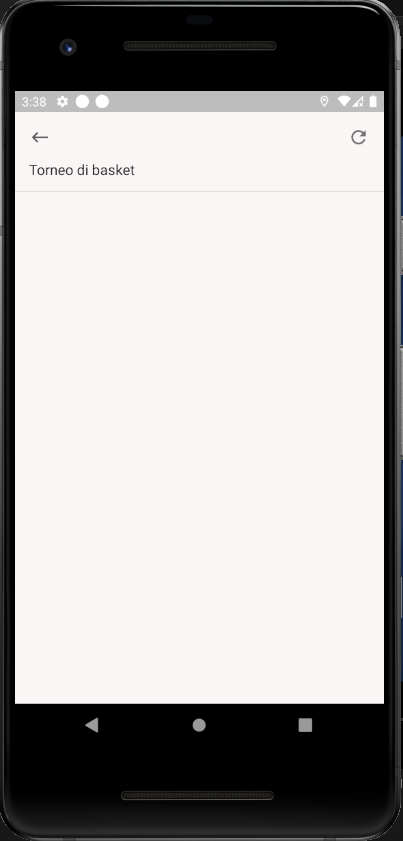
\includegraphics[width=0.4\textwidth]{images/app/live/live_overview}
    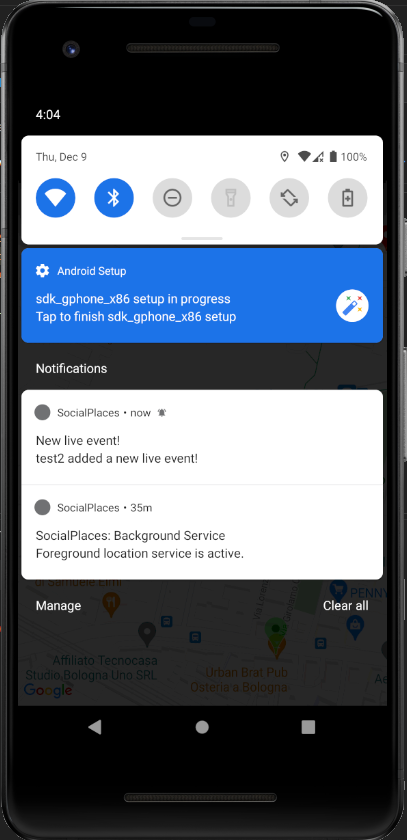
\includegraphics[width=0.4\textwidth]{images/app/notification/live/notifed_live}
    \caption{On the left, the \textbf{Live events} screen. On the right, the notification of a new live event added.}
\end{figure}
\end{document}